% Created 2019-08-22 jue 19:01
\documentclass[a4paper]{scrartcl}
\usepackage[utf8]{inputenc}
\usepackage[T1]{fontenc}
\usepackage{fixltx2e}
\usepackage{graphicx}
\usepackage{longtable}
\usepackage{float}
\usepackage{wrapfig}
\usepackage{rotating}
\usepackage[normalem]{ulem}
\usepackage{amsmath}
\usepackage{textcomp}
\usepackage{marvosym}
\usepackage{wasysym}
\usepackage{amssymb}
\usepackage{hyperref}
\tolerance=1000
\usepackage{khpreamble}
\usepackage{subfigure}
\author{Kjartan Halvorsen}
\date{\today}
\title{Harddisk drive control design exercise (Å\&W ex 1.2)}
\hypersetup{
  pdfkeywords={},
  pdfsubject={},
  pdfcreator={Emacs 25.3.50.2 (Org mode 8.2.10)}}
\begin{document}

\maketitle


\section*{The closed-loop transfer functions}
\label{sec-1}
\begin{center}
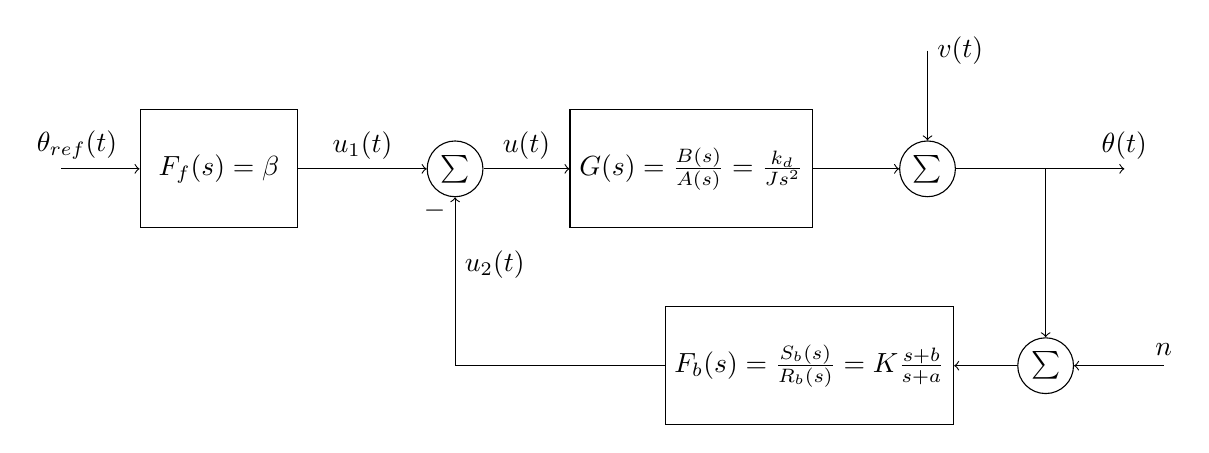
\begin{tikzpicture}
\tikzset{node distance=2cm, 
    block/.style={rectangle, draw, minimum height=15mm, minimum width=20mm},
    sumnode/.style={circle, draw, inner sep=2pt}        
}

  \node[coordinate] (input) {};
  \node[block, right of=input] (TR) {$F_f(s)=\beta$};
  \node[sumnode, right of=TR, node distance=30mm] (sum) {$\sum$};
  \node[block,right of=sum, node distance=30mm] (plant) {$G(s)=\frac{B(s)}{A(s)}=\frac{k_d}{Js^2}$};
  \node[sumnode, right of=plant, node distance=30mm] (sumdist) {$\sum$};
  \node[coordinate, above of=sumdist, node distance=15mm] (dist) {};
  \node[coordinate, right of=sumdist, node distance=15mm] (measure) {};
  \node[coordinate, right of=measure, node distance=10mm] (output) {};
  \node[sumnode,below of=measure, node distance=25mm] (sumnoise) {$\sum$};
  \node[coordinate, right of=sumnoise, node distance=15mm] (noise) {};
  \node[block,left of=sumnoise, node distance=30mm] (SR) {$F_b(s) = \frac{S_b(s)}{R_b(s)}= K\frac{s+b}{s+a}$};

  \draw[->] (input) -- node[above, pos=0.2] {$\theta_{ref}(t)$} (TR);
  \draw[->] (TR) -- node[above] {$u_1(t)$} (sum);
  \draw[->] (sum) -- node[above] {$u(t)$} (plant);
  \draw[->] (plant) -- (sumdist);
  \draw[->] (dist) -- node[at start, right] {$v(t)$} (sumdist);
  \draw[->] (sumdist) -- node[at end, above] {$\theta(t)$} (output);
  \draw[->] (measure) -- (sumnoise);
  \draw[->] (noise) -- node[at start, above] {$n$} (sumnoise);
  \draw[->] (sumnoise) -- (SR);
  \draw[->] (SR) -| (sum) node[right, pos=0.8] {$u_2(t)$} node[left, pos=0.96] {$-$};
\end{tikzpicture}
\end{center}

\begin{enumerate}
\item \textbf{Show that the closed-loop system from the three input signals $\theta_{ref}(t)$, $v(t)$ and $n(t)$ is given by}
     \[ \Theta(s) = \frac{G(s)F_f(s)}{1 + G(s)F_b(s)}\Theta_{ref}(s) + \underbrace{\frac{1}{1 + G(s)F_b(s)}}_{S(s)}V(s) - \underbrace{\frac{G(s)F_b(s)}{1 + G(s)F_b(s)}}_{T(s)}N(s) \]
\item \textbf{Show that \( S(s) + T(s) = 1\)}
\end{enumerate}

\section*{The characteristic equation}
\label{sec-2}
\textbf{Show that the characteristic equation for the closed-loop system is}
\begin{equation}
A(s)R_b(s) + B(s)S_b(s) = s^3 + as^2 + \frac{Kk_d}{J}s + \frac{Kk_d}{J}b = 0.
\label{eq:chareq}
\end{equation}

\section*{Desired closed-loop poles}
\label{sec-3}
The closed-loop system is of order three, so there are three poles to specify. Assume that the specification on the speed of the response of the closed-loop system requires the poles to be at a distance of \(\omega_0\) from the origin. \textbf{Sketch suitable positions of the three poles in the s-plane below.}
\begin{center}
\begin{tikzpicture}

  \draw[->] (-3,0) to (3,0) node[below] {Re};
  \draw[->] (0,-3) to (0,3) node[right] {Im};

  \draw[thin,dashed] (0,0) circle [radius=2cm];

  %\draw[->, dashed] (0,0) -- node[above right, pos=0.8] {$r=\omega_0$} (140:2) ;

  \node at (-2,-0.3) {$-\omega_0$};
  \node at (0.4,2) {$i\omega_0$};
  \node at (0.4,-2) {$-i\omega_0$};
\end{tikzpicture}
\end{center}

\section*{Determine the controller parameters}
\label{sec-4}
A suitable set of three closed-loop poles is obtained as the roots of the characteristic polynomial
\begin{equation}
s^3 + 2\omega_0s^2 + 2\omega_0^2s + \omega_0^3.
\label{eq:desired}
\end{equation}
By comparing the characteristic polynomial in \eqref{eq:chareq} to the desired polynomial in \eqref{eq:desired}, we can determine the controller parameters. \textbf{Find the parameters of the feedback controller.}
\begin{flalign*}
a &= & \\[3mm]
b &= \\[3mm]
K &= 
\end{flalign*}

\section*{Root locus}
\label{sec-5}
Consider the closed-loop characteristic equation \(1 + K\frac{s+b}{s^2(s+a)} = 0\) using the values for $a$ and $b$ found above (but leave $K>0$ undetermined). \textbf{Draw the root locus w.r.t the controller gain $K$.}
\begin{center}
 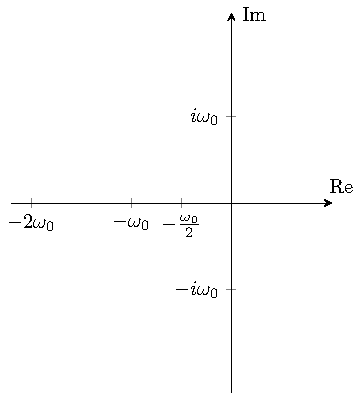
\includegraphics[]{../figures/implane-rlocus}
\end{center}
\textbf{Is \(F_b(s) = K \frac{s+b}{s+a}\) a \emph{lead-compensator} or a \emph{lag-compensator}?}

\section*{The loop gain}
\label{sec-6}
Show that the loop gain of the closed-loop system is
\[G_o(s) = G(s)F_b(s) = \frac{\omega_0^2(2s + \omega_0)}{s^2(s+2\omega_0)}.\]

\textbf{Determine and mark the (amplitude) crossover frequency $\omega_c$, the phase-crossover frequency $\omega_p$, the phase margin $\varphi_m$ and the gain margin $A_m$ in the bodeplot of the loop gain below.}
\begin{center}
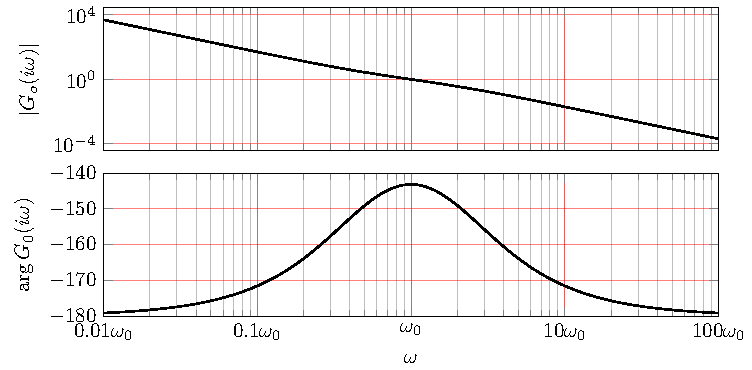
\includegraphics[]{../figures/bode-loop-gain}
\end{center}


\section*{The set-point weighting}
\label{sec-7}
The closed-loop transfer function from reference signal to output is 
\[ G_c(s) = \frac{G(s)F_f(s)}{1 + G(s)F_b(s)} = \frac{\beta \frac{k_d/J}{s^2}}{ 1 + \frac{k_d/J}{s^2} K \frac{s+b}{s+a}} = \frac{\beta \frac{k_d}{J} (s+a)}{s^2(s+a) + K\frac{k_d}{J}(s+b)}.\]
Determine $\beta$ such that the closed-loop transfer function has unit static gain (\(G_c(0)=1\)).

\section*{Discretizing the controller}
\label{sec-8}
The control law is 
\begin{align*} 
U(s) &= F_f(s)\Theta_{ref}(s) - F_b(s)\Theta(s)\\
 &= \underbrace{\beta\Theta_{ref}(s)}_{U_1(s)} - \underbrace{K\frac{s + b}{s+a} \Theta(s)}_{U_2(s)}
\end{align*}
which means that it an be written in the time-domain as \(u(t) = u_1(t) - u_2(t)\), where
\begin{equation}
  u_1(t) = \beta \theta_{ref}(t),
\end{equation}
and the output feedback $u_2(t)$ is 
\[U_2(s) = K \cdot \frac{s + b}{s + a} \Theta(s)\]
which be written as the ODE 
$$\dot{u}_2 + a u_2 =  K (\dot{\theta} + b \theta).$$
The term \(u_1(t)\) is straightforward to discretize as
$$ u_1(t) = \beta \theta_{ref}(t) \quad \Rightarrow \quad u_1(kh) = \beta \theta_{ref}(kh). $$
The second term $u_2(t)$ requires a discrete approximation of the derivative. There are a number of different alternatives. The simplest is the Euler forward approximation
$$ \dot{x}(t) = \frac{dx}{dt} \approx \frac{x(t+h) - x(t)}{h}, $$
where $h$ is the sampling interval. 
\textbf{Show that the Euler forward approximation gives} 
$$ u_2(kh+h) = ( 1 - ah) u_2(kh) + K \Big(\theta(kh+h) + (1-bh)\theta(kh)\Big). $$
\textbf{For which values of $h$ is the discretized feedback controller a stable system?}
% Emacs 25.3.50.2 (Org mode 8.2.10)
\end{document}